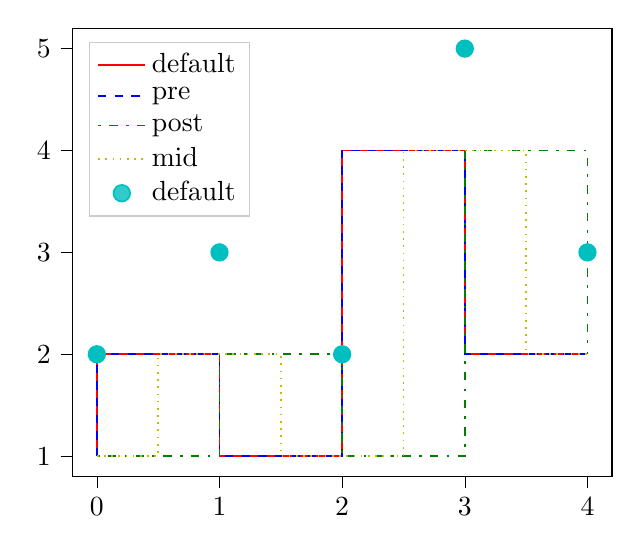
\begin{tikzpicture}

\definecolor{darkgray176}{RGB}{176,176,176}
\definecolor{darkturquoise0191191}{RGB}{0,191,191}
\definecolor{goldenrod1911910}{RGB}{191,191,0}
\definecolor{green01270}{RGB}{0,127,0}
\definecolor{lightgray204}{RGB}{204,204,204}

\begin{axis}[
legend cell align={left},
legend style={
  fill opacity=0.8,
  draw opacity=1,
  text opacity=1,
  at={(0.03,0.97)},
  anchor=north west,
  draw=lightgray204
},
tick align=outside,
tick pos=left,
x grid style={darkgray176},
xmin=-0.2, xmax=4.2,
xtick style={color=black},
y grid style={darkgray176},
ymin=0.8, ymax=5.2,
ytick style={color=black}
]
\addplot [semithick, red, const plot mark right]
table {%
0 1
1 2
2 1
3 4
4 2
};
\addlegendentry{default}
\addplot [semithick, blue, const plot mark right, dashed]
table {%
0 1
1 2
2 1
3 4
4 2
};
\addlegendentry{pre}
\addplot [semithick, green01270, const plot mark left, dash pattern=on 1pt off 3pt on 3pt off 3pt]
table {%
0 1
1 2
2 1
3 4
4 2
};
\addlegendentry{post}
\addplot [semithick, goldenrod1911910, const plot mark mid, dotted]
table {%
0 1
1 2
2 1
3 4
4 2
};
\addlegendentry{mid}
\addplot [semithick, darkturquoise0191191, mark=*, mark size=3, mark options={solid}, only marks]
table {%
0 2
1 3
2 2
3 5
4 3
};
\addlegendentry{default}
\end{axis}

\end{tikzpicture}
